\documentclass[14pt,a4paper,report]{report}
\usepackage[a4paper, mag=1000, left=2.5cm, right=1cm, top=2cm, bottom=2cm, headsep=0.7cm, footskip=1cm]{geometry}
\usepackage[utf8]{inputenc}
\usepackage[english,russian]{babel}
\usepackage{indentfirst}
\usepackage[dvipsnames]{xcolor}
\usepackage[colorlinks]{hyperref}
\usepackage{listings} 
\usepackage{fancyhdr}
\usepackage{caption}
\usepackage{amsmath}
\usepackage{latexsym}
\usepackage{graphicx}
\usepackage{amsmath}
\usepackage{booktabs}
\usepackage{array}
\hypersetup{
	colorlinks = true,
	linkcolor  = black
}

\usepackage{titlesec}
\titleformat{\chapter}
{\Large\bfseries} % format
{}                % label
{0pt}             % sep
{\huge}           % before-code


\DeclareCaptionFont{white}{\color{white}} 

% Listing description
\usepackage{listings} 
\DeclareCaptionFormat{listing}{\colorbox{gray}{\parbox{\textwidth}{#1#2#3}}}
\captionsetup[lstlisting]{format=listing,labelfont=white,textfont=white}
\lstset{ 
	% Listing settings
	inputencoding = utf8,			
	extendedchars = \true, 
	keepspaces = true, 			  	 % Поддержка кириллицы и пробелов в комментариях
	language = C++,            	 	 % Язык программирования (для подсветки)
	basicstyle = \small\sffamily, 	 % Размер и начертание шрифта для подсветки кода
	numbers = left,               	 % Где поставить нумерацию строк (слева\справа)
	numberstyle = \tiny,          	 % Размер шрифта для номеров строк
	stepnumber = 1,               	 % Размер шага между двумя номерами строк
	numbersep = 5pt,              	 % Как далеко отстоят номера строк от подсвечиваемого кода
	backgroundcolor = \color{white}, % Цвет фона подсветки - используем \usepackage{color}
	showspaces = false,           	 % Показывать или нет пробелы специальными отступами
	showstringspaces = false,    	 % Показывать или нет пробелы в строках
	showtabs = false,           	 % Показывать или нет табуляцию в строках
	frame = single,              	 % Рисовать рамку вокруг кода
	tabsize = 2,                  	 % Размер табуляции по умолчанию равен 2 пробелам
	captionpos = t,             	 % Позиция заголовка вверху [t] или внизу [b] 
	breaklines = true,           	 % Автоматически переносить строки (да\нет)
	breakatwhitespace = false,   	 % Переносить строки только если есть пробел
	escapeinside = {\%*}{*)}      	 % Если нужно добавить комментарии в коде
}

\begin{document}

\def\contentsname{Содержание}

% Titlepage
\begin{titlepage}
	\begin{center}
		\textsc{Санкт-Петербургский Политехнический 
			Университет Петра Великого\\[5mm]
			Кафедра компьютерных систем и программных технологий}
		
		\vfill
		
		\textbf{Отчёт по лабораторной работе №4\\[3mm]
			Курс: «Администрирование компьютерных сетей»\\[3mm]
			Тема: «Устранение уязвимостей»\\[35mm]
			}
	\end{center}
	
	\hfill
	\begin{minipage}{.5\textwidth}
		Выполнил студент:\\[2mm] 
		Бояркин Никита Сергеевич\\
		Группа: 13541/3\\[5mm]
		
		Проверил:\\[2mm] 
		Малышев Игорь Алексеевич
	\end{minipage}
	\vfill
	\begin{center}
		Санкт-Петербург\\ \the\year\ г.
	\end{center}
\end{titlepage}

% Contents
\tableofcontents
\clearpage

\chapter{Лабораторная работа №4}

\section{Цель работы}

Получить навыки работы с Netfilter, используя iptables -- утилита для управления межсетевым экраном.

\section{Устранение уязвимостей}

Уязвимости, найденные в предыдущих лабораторных работах связаны в первую очередь с открытыми портами. Утилита iptables позволяет задать правила для входящих/исходящих tcp/udp портов для обеспечения безопасности.

Чтобы показать все правила, необходимо ввести команду:

\begin{figure}[h!]
	\centering
	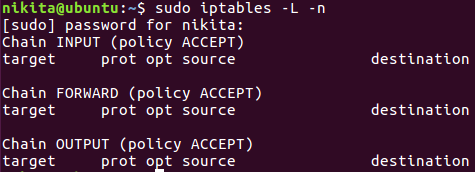
\includegraphics[scale = 1.15]{images/1.png}
	\caption{Правила по-умолчанию}
	\label{image:1}
\end{figure}

По-умолчанию нет никаких правил, а следовательно все внешние порты закрыты.

Открытие TCP порта 80 производится следующей командой:

\begin{figure}[h!]
	\centering
	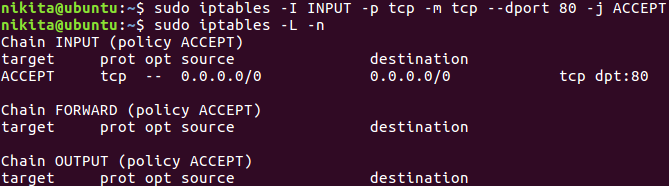
\includegraphics[scale = 0.95]{images/2.png}
	\caption{Создание нового правила открытия 80 tcp порта}
	\label{image:2}
\end{figure}

\clearpage

Удаление правила по его порядковому номеру в таблице производится следующей командой:

\begin{figure}[h!]
	\centering
	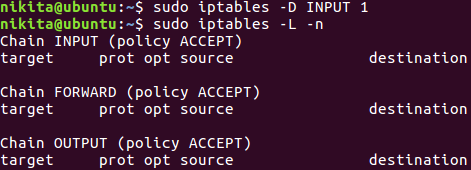
\includegraphics[scale = 1.25]{images/3.png}
	\caption{Удаление правила по номеру}
	\label{image:3}
\end{figure}

Удаление всех правил производится следующей командой:

\begin{figure}[h!]
	\centering
	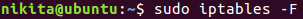
\includegraphics[scale = 1.35]{images/4.png}
	\caption{Удаление всех правил}
	\label{image:4}
\end{figure}

Запрет исходящих соединений на конкретный адрес:

\begin{figure}[h!]
	\centering
	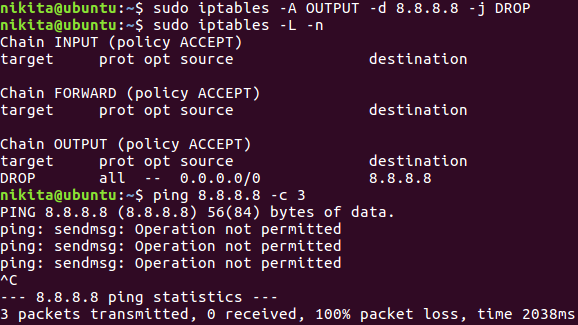
\includegraphics[scale = 1.05]{images/5.png}
	\caption{Запрет исходящих соединений на конкретный адрес}
	\label{image:5}
\end{figure}

Также есть возможность сохранить и восстановить правила:

\begin{figure}[h!]
	\centering
	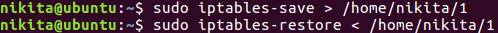
\includegraphics[scale = 1.25]{images/6.png}
	\caption{Сохранение и восстановление правил из файла}
	\label{image:6}
\end{figure}

\section{Вывод}

Межсетевой экран, встроенный в ядро Linux, называется Netfilter, а iptables -- утилита для управления этим межсетевым экраном.

В системе netfilter пакеты пропускаются через цепочки. Цепочка является упорядоченным списком правил, а каждое правило может содержать критерии и действие или переход.

Утилита iptables позволяет легко получить доступ к межсетевому экрану, однако большое количество флагов не всегда позволяет удобно ей пользоваться. В этом плане брандмауэр Windows более интуитивно понятно позволяет задавать правила.




\end{document}